\RequirePackage[l2tabu, orthodox]{nag}

\documentclass{article}

\usepackage[utf8]{inputenc}
\usepackage[ngerman]{babel}

\usepackage{natbib}
\usepackage{graphicx}
\usepackage{capt-of}
\usepackage[colorlinks,pdfpagelabels,pdfstartview=FitH,bookmarksopen=true,bookmarksnumbered=true,linkcolor=black,plainpages=false,hypertexnames=false,citecolor=black]{hyperref}
\usepackage{caption}
\usepackage{subfigure}
\usepackage{listings}
\usepackage{microtype}

% http://tex.stackexchange.com/questions/167948/package-rerunfilecheck-warning-file-out-has-changed
\usepackage{bookmark}

% gantt charts: http://ctan.mirrorcatalogs.com/graphics/pgf/contrib/pgfgantt/pgfgantt.pdf
\usepackage{pgfgantt}

% change margins to 2.5 cm and enable landscape
\usepackage[margin=3cm]{geometry}
\usepackage{pdflscape}

\usepackage{tabulary}

% place figures at exactly the position given in the code
\usepackage{float}

% custom counters for lists
\usepackage{enumitem}

\newcommand{\appname}{Flashcard-Website}


\begin{document}
\begin{titlepage}
    \large
    \begin{flushleft}
        Web Engineering, 2. Semester \\
        Projektmanagment, 2. Semester \\
        TINF13B2
    \end{flushleft}
    
    \vfill

    \begin{center}
    	% H. Balzert, Lehrbuch der Software-Technik
        \Huge SOLL-/IST-Analyse\\
        \Large \appname \\
        \vspace{1cm}
        \normalsize David Ehlen (5460297),\\
        Julien Hadley Jack (4739854), \\
        Sebastian Dernbach (9586963), \\
        \vspace\medskipamount
        \vspace\medskipamount
        Karlsruhe, 07.07.2014
    \end{center}
    
    \vfill
    
    \begin{flushright}
        Duale Hochschule \\
        Baden-Württemberg \\
        \vspace\medskipamount
        Betreuer: Jörn Eisenbiegler,\\
        Simone Freudenmann
    \end{flushright}
\end{titlepage}

\newpage

% removes the page numbers for the toc
\pagestyle{empty}
\addtocontents{toc}{\protect\thispagestyle{empty}}
\tableofcontents
\cleardoublepage

% normal page numbering for the rest of the document
\setcounter{page}{1}
\pagestyle{plain}
\setcounter{page}{1}

\section{Projektstrukturplan}
\subsection{Zielbestimmung}
Das Endprodukt setzt alle Musskriterien um. Außerdem wurden noch drei Wunschkriterien erfüllt:
\begin{description}
	\item[/WK10/] Für jedes Karteikartenset werden Statistiken angezeigt (Erfolgsquote,...).
	\item[/WK20/] Mathematische Ausdrücke werden in natürlicher Form (z.b. \( e^{\frac{3}{4}\pi i}\)) dargestellt.
	\item[/WK30/]\label{bilder} Bilder können eingefügt werden.
\end{description}

\noindent Hierbei kann man bei \textbf{/WK30/} nur Bilder über die URL einbetten, aber nicht neue Bilder zu dem Server hochladen.

\subsection{Nichtfunktionale Anforderungen}
Die nichtfunktionalen Anforderungen wurden soweit wie möglich getestet.

\subsection{Testfälle}
Die Testfälle der Musskriterien und erfüllten Wunschkriterien wurden mit verschiedenen Browser getestet. Dies hat uns geholfen einige Fehler noch zu finden. Unterschiede zwischen z.B. Google Chrome und Mozilla Firefox führten zu unterschiedlichen Darstellungen. Wenn möglich wurde dies behoben.

\section{Terminplan}
Wir haben uns für Amazon AWS entschieden zur Bereitstellung des Servers. Dies ermöglicht eine einfache Kollaboration zwischen den Mitarbeitern und lässt die Webseite mit der Anzahl der Besucher skalieren. Dieser Dienst wird auch von Firmen wie NASA, Pinterest und Netflix für ihre produktiven Dienste benutzt.

Dabei hatten wir mit komplexeren Themen wie Firewallregeln und Benutzerverwaltung öfters Probleme. Diese waren nicht eingeplant, so dass das Projektende um 2 Tage überschritten wurde. Da aber ein Puffer zwischen Projektende und Abgabetermin der Dokumentation mitkalkuliert war, konnte dieser Termin ohne Schwierigkeiten eingehalten werden.


\section{Ressourcenplan}
Die Zusammenarbeit zwischen den Mitgliedern des Projektes hat gut funktioniert. Ein Vorteil war, dass sich die Studenten während der Projektphase in ihrer Theoriephase befanden. Das bedeutet, dass sie sich täglich gesehen haben und dadurch oft über ihren Stand und ihre Problemen ausgetauscht haben.

\smallskip
\noindent Es gab keine Ausfälle von Arbeitskräften durch Krankheiten oder aus anderen Gründen.

\smallskip
\noindent Das Projekt konnte mit den geplanten Ressourcen umgesetzt werden.

\section{Kostenplan}
Während des Projektes erhielt der Miterarbeiter, der für die Serveradministration zuständig war, eine E-Mail von Amazon. Es enthielt eine Warnung wegen verdächtigen Aktivitäten auf dem Amazon-AWS-Account. Der Mitarbeiter hat danach beim Überprüfen Änderungen von einer unerlaubten Drittperson auf dem Account entdeckt.

Nach einer mehrstündigen Fehlersuche konnte der Weg festgestellt werden, wie diese Person Zugang erlangen konnte: 

Der Code des Projektes war in einem öffentlichen Versionskontrollsystem auf www.github.com veröffentlicht. Die Datei mit den nötigen Login-Daten für das Amazon-AWS-Account wurde einem Filter hinzugefügt, damit sie nicht veröffentlicht wird. Ein Mitarbeiter hatte Software verwendet, um seine Änderungen dem Versionskontrollsystem hinzuzufügen, die diesen Filter nicht benutzte.

Da Amazon AWS für kleine bis riesigen Webseiten verwendet werden kann, gibt es auch kostenpflichtige Optionen. Die unerlaubte Person hat eine Vielzahl von den Optionen dazugebucht. Obwohl er nur Zugriff für einen Tag hatte, konnte er eine Rechnung von 568,14 USD in dieser Zeit für den Mitarbeiter ansammeln.

\begin{figure}[H]
    \centering
    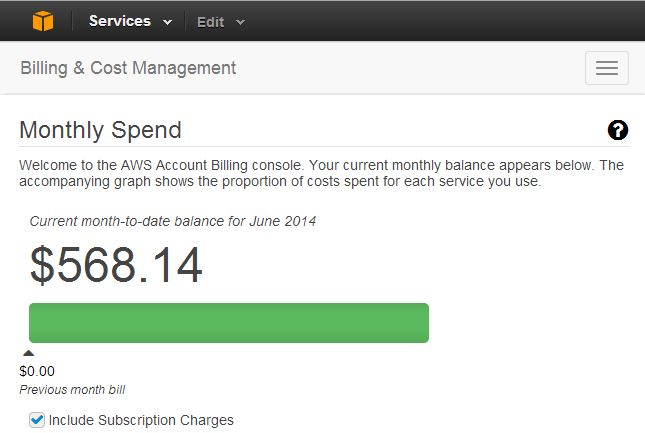
\includegraphics[width=0.7\textwidth]{images/amazon-bill.jpg}
    \caption{Rechnung Amazon AWS}
    \label{fig:bill}
\end{figure}



\section{Risikoplan}

\section{Kommunikationsplan}

\section{Persönliche Einschätzung}
\begin{figure}[H]
    \centering
    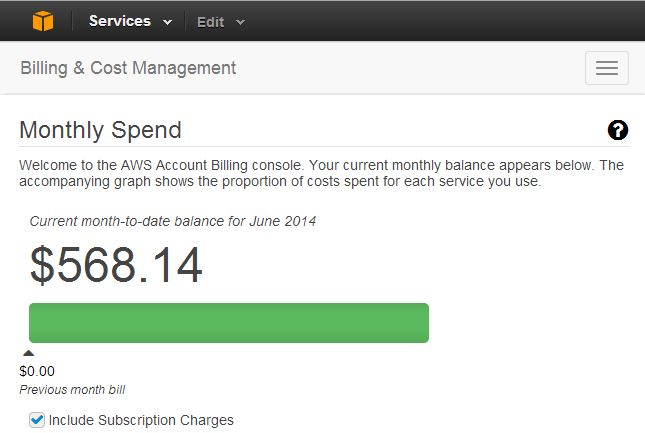
\includegraphics[width=0.7\textwidth]{images/amazon-bill.jpg}
    \caption{Rechnung Amazon AWS}
    \label{fig:bill}
\end{figure}

\section{Ehrenamtliche Erklärung}

Ich erkläre ehrenwörtlich,
\begin{itemize}
    \item dass ich meine Projektarbeit selbständig geplant und durchgeführt habe;
    \item dass ich die Übernahme wörtlicher Zitate aus der Literatur sowie die Verwendung der Gedanken anderer Autoren an den entsprechenden Stellen innerhalb der Arbeit gekennzeichnet habe;
    \item dass ich meine Projektarbeit bei keiner anderen Prüfung
    vorgelegt habe.
\end{itemize}
Ich bin mir bewusst, dass eine falsche Erklärung rechtliche Folgen haben wird. \\

\vspace{1cm}
Karlsruhe, 05.07.2014 

\end{document}